% Created by tikzDevice version 0.10.1 on 2016-09-09 19:46:08
% !TEX encoding = UTF-8 Unicode
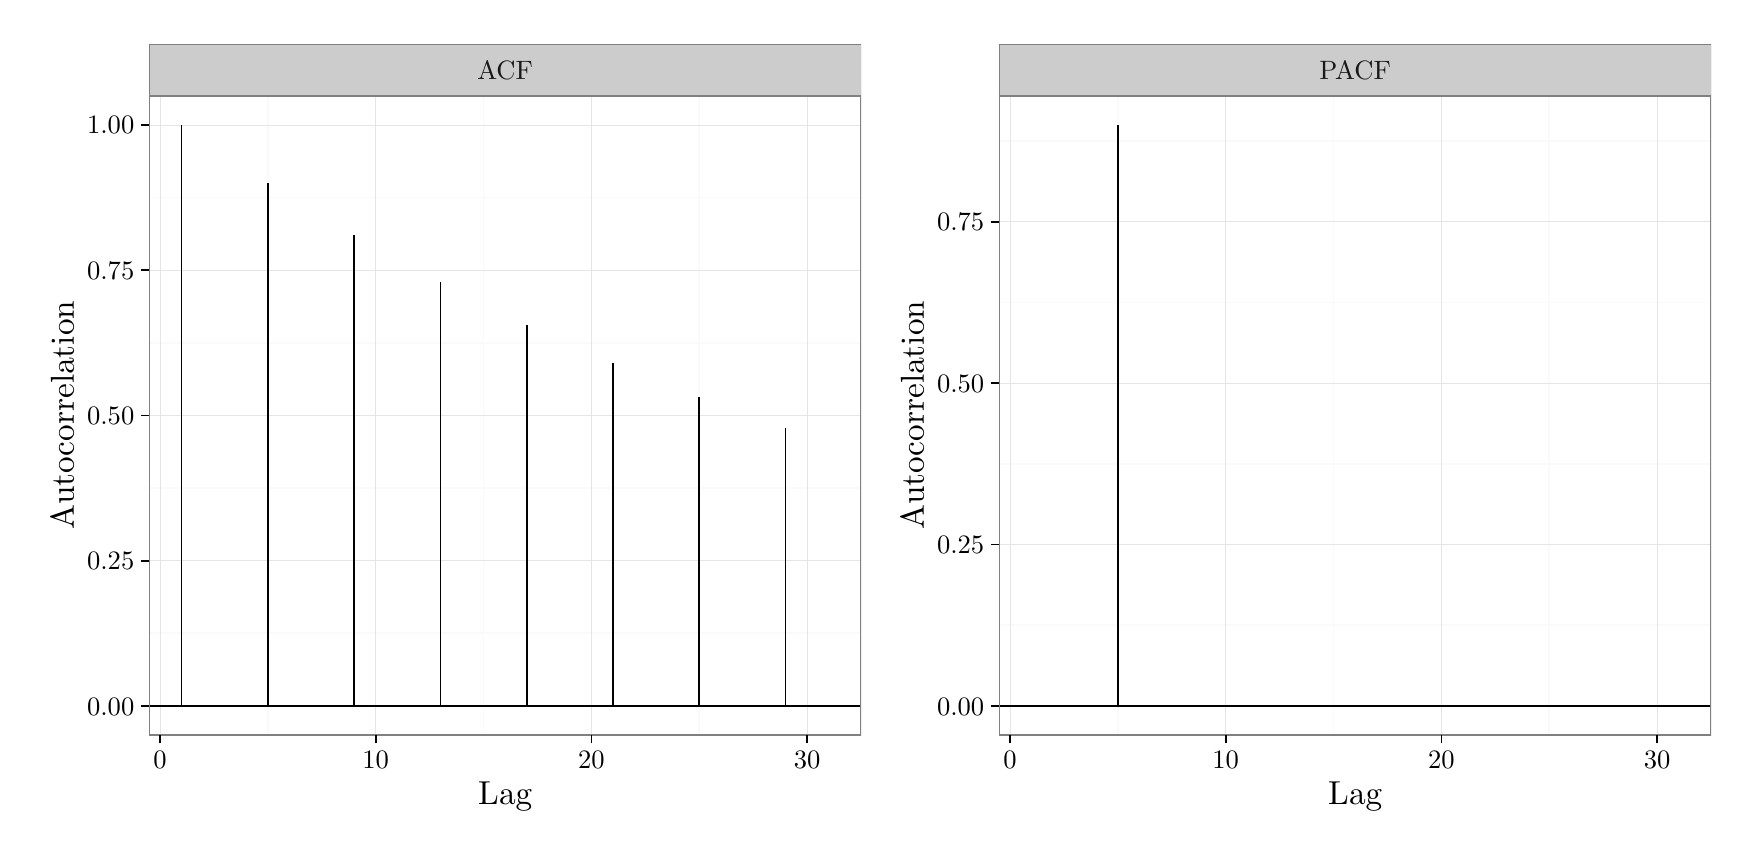
\begin{tikzpicture}[x=1pt,y=1pt]
\definecolor{fillColor}{RGB}{255,255,255}
\path[use as bounding box,fill=fillColor,fill opacity=0.00] (0,0) rectangle (614.29,289.08);
\begin{scope}
\path[clip] (  0.00,  0.00) rectangle (307.15,289.08);
\definecolor{drawColor}{RGB}{255,255,255}
\definecolor{fillColor}{RGB}{255,255,255}

\path[draw=drawColor,line width= 0.6pt,line join=round,line cap=round,fill=fillColor] ( -0.00,  0.00) rectangle (307.15,289.08);
\end{scope}
\begin{scope}
\path[clip] ( 43.93, 33.48) rectangle (301.15,264.47);
\definecolor{fillColor}{RGB}{255,255,255}

\path[fill=fillColor] ( 43.93, 33.48) rectangle (301.15,264.47);
\definecolor{drawColor}{gray}{0.98}

\path[draw=drawColor,line width= 0.6pt,line join=round] ( 43.93, 70.23) --
	(301.15, 70.23);

\path[draw=drawColor,line width= 0.6pt,line join=round] ( 43.93,122.72) --
	(301.15,122.72);

\path[draw=drawColor,line width= 0.6pt,line join=round] ( 43.93,175.22) --
	(301.15,175.22);

\path[draw=drawColor,line width= 0.6pt,line join=round] ( 43.93,227.72) --
	(301.15,227.72);

\path[draw=drawColor,line width= 0.6pt,line join=round] ( 86.80, 33.48) --
	( 86.80,264.47);

\path[draw=drawColor,line width= 0.6pt,line join=round] (164.74, 33.48) --
	(164.74,264.47);

\path[draw=drawColor,line width= 0.6pt,line join=round] (242.69, 33.48) --
	(242.69,264.47);
\definecolor{drawColor}{gray}{0.90}

\path[draw=drawColor,line width= 0.2pt,line join=round] ( 43.93, 43.98) --
	(301.15, 43.98);

\path[draw=drawColor,line width= 0.2pt,line join=round] ( 43.93, 96.47) --
	(301.15, 96.47);

\path[draw=drawColor,line width= 0.2pt,line join=round] ( 43.93,148.97) --
	(301.15,148.97);

\path[draw=drawColor,line width= 0.2pt,line join=round] ( 43.93,201.47) --
	(301.15,201.47);

\path[draw=drawColor,line width= 0.2pt,line join=round] ( 43.93,253.97) --
	(301.15,253.97);

\path[draw=drawColor,line width= 0.2pt,line join=round] ( 47.82, 33.48) --
	( 47.82,264.47);

\path[draw=drawColor,line width= 0.2pt,line join=round] (125.77, 33.48) --
	(125.77,264.47);

\path[draw=drawColor,line width= 0.2pt,line join=round] (203.72, 33.48) --
	(203.72,264.47);

\path[draw=drawColor,line width= 0.2pt,line join=round] (281.66, 33.48) --
	(281.66,264.47);
\definecolor{drawColor}{RGB}{0,0,0}

\path[draw=drawColor,line width= 0.6pt,line join=round] ( 43.93, 43.98) -- (301.15, 43.98);

\path[draw=drawColor,line width= 0.6pt,line join=round] ( 55.62,253.97) -- ( 55.62, 43.98);

\path[draw=drawColor,line width= 0.6pt,line join=round] ( 63.41, 43.98) -- ( 63.41, 43.98);

\path[draw=drawColor,line width= 0.6pt,line join=round] ( 71.21, 43.98) -- ( 71.21, 43.98);

\path[draw=drawColor,line width= 0.6pt,line join=round] ( 79.00, 43.98) -- ( 79.00, 43.98);

\path[draw=drawColor,line width= 0.6pt,line join=round] ( 86.80,232.97) -- ( 86.80, 43.98);

\path[draw=drawColor,line width= 0.6pt,line join=round] ( 94.59, 43.98) -- ( 94.59, 43.98);

\path[draw=drawColor,line width= 0.6pt,line join=round] (102.39, 43.98) -- (102.39, 43.98);

\path[draw=drawColor,line width= 0.6pt,line join=round] (110.18, 43.98) -- (110.18, 43.98);

\path[draw=drawColor,line width= 0.6pt,line join=round] (117.98,214.07) -- (117.98, 43.98);

\path[draw=drawColor,line width= 0.6pt,line join=round] (125.77, 43.98) -- (125.77, 43.98);

\path[draw=drawColor,line width= 0.6pt,line join=round] (133.56, 43.98) -- (133.56, 43.98);

\path[draw=drawColor,line width= 0.6pt,line join=round] (141.36, 43.98) -- (141.36, 43.98);

\path[draw=drawColor,line width= 0.6pt,line join=round] (149.15,197.06) -- (149.15, 43.98);

\path[draw=drawColor,line width= 0.6pt,line join=round] (156.95, 43.98) -- (156.95, 43.98);

\path[draw=drawColor,line width= 0.6pt,line join=round] (164.74, 43.98) -- (164.74, 43.98);

\path[draw=drawColor,line width= 0.6pt,line join=round] (172.54, 43.98) -- (172.54, 43.98);

\path[draw=drawColor,line width= 0.6pt,line join=round] (180.33,181.75) -- (180.33, 43.98);

\path[draw=drawColor,line width= 0.6pt,line join=round] (188.13, 43.98) -- (188.13, 43.98);

\path[draw=drawColor,line width= 0.6pt,line join=round] (195.92, 43.98) -- (195.92, 43.98);

\path[draw=drawColor,line width= 0.6pt,line join=round] (203.72, 43.98) -- (203.72, 43.98);

\path[draw=drawColor,line width= 0.6pt,line join=round] (211.51,167.97) -- (211.51, 43.98);

\path[draw=drawColor,line width= 0.6pt,line join=round] (219.30, 43.98) -- (219.30, 43.98);

\path[draw=drawColor,line width= 0.6pt,line join=round] (227.10, 43.98) -- (227.10, 43.98);

\path[draw=drawColor,line width= 0.6pt,line join=round] (234.89, 43.98) -- (234.89, 43.98);

\path[draw=drawColor,line width= 0.6pt,line join=round] (242.69,155.57) -- (242.69, 43.98);

\path[draw=drawColor,line width= 0.6pt,line join=round] (250.48, 43.98) -- (250.48, 43.98);

\path[draw=drawColor,line width= 0.6pt,line join=round] (258.28, 43.98) -- (258.28, 43.98);

\path[draw=drawColor,line width= 0.6pt,line join=round] (266.07, 43.98) -- (266.07, 43.98);

\path[draw=drawColor,line width= 0.6pt,line join=round] (273.87,144.41) -- (273.87, 43.98);

\path[draw=drawColor,line width= 0.6pt,line join=round] (281.66, 43.98) -- (281.66, 43.98);

\path[draw=drawColor,line width= 0.6pt,line join=round] (289.46, 43.98) -- (289.46, 43.98);
\definecolor{drawColor}{gray}{0.50}

\path[draw=drawColor,line width= 0.6pt,line join=round,line cap=round] ( 43.93, 33.48) rectangle (301.15,264.47);
\end{scope}
\begin{scope}
\path[clip] ( 43.93,264.47) rectangle (301.15,283.08);
\definecolor{drawColor}{gray}{0.50}
\definecolor{fillColor}{gray}{0.80}

\path[draw=drawColor,line width= 0.2pt,line join=round,line cap=round,fill=fillColor] ( 43.93,264.47) rectangle (301.15,283.08);
\definecolor{drawColor}{gray}{0.10}

\node[text=drawColor,anchor=base,inner sep=0pt, outer sep=0pt, scale=  0.96] at (172.54,270.47) {ACF};
\end{scope}
\begin{scope}
\path[clip] (  0.00,  0.00) rectangle (614.29,289.08);
\definecolor{drawColor}{RGB}{0,0,0}

\node[text=drawColor,anchor=base east,inner sep=0pt, outer sep=0pt, scale=  0.96] at ( 38.53, 40.67) {0.00};

\node[text=drawColor,anchor=base east,inner sep=0pt, outer sep=0pt, scale=  0.96] at ( 38.53, 93.17) {0.25};

\node[text=drawColor,anchor=base east,inner sep=0pt, outer sep=0pt, scale=  0.96] at ( 38.53,145.67) {0.50};

\node[text=drawColor,anchor=base east,inner sep=0pt, outer sep=0pt, scale=  0.96] at ( 38.53,198.16) {0.75};

\node[text=drawColor,anchor=base east,inner sep=0pt, outer sep=0pt, scale=  0.96] at ( 38.53,250.66) {1.00};
\end{scope}
\begin{scope}
\path[clip] (  0.00,  0.00) rectangle (614.29,289.08);
\definecolor{drawColor}{RGB}{0,0,0}

\path[draw=drawColor,line width= 0.6pt,line join=round] ( 40.93, 43.98) --
	( 43.93, 43.98);

\path[draw=drawColor,line width= 0.6pt,line join=round] ( 40.93, 96.47) --
	( 43.93, 96.47);

\path[draw=drawColor,line width= 0.6pt,line join=round] ( 40.93,148.97) --
	( 43.93,148.97);

\path[draw=drawColor,line width= 0.6pt,line join=round] ( 40.93,201.47) --
	( 43.93,201.47);

\path[draw=drawColor,line width= 0.6pt,line join=round] ( 40.93,253.97) --
	( 43.93,253.97);
\end{scope}
\begin{scope}
\path[clip] (  0.00,  0.00) rectangle (614.29,289.08);
\definecolor{drawColor}{RGB}{0,0,0}

\path[draw=drawColor,line width= 0.6pt,line join=round] ( 47.82, 30.48) --
	( 47.82, 33.48);

\path[draw=drawColor,line width= 0.6pt,line join=round] (125.77, 30.48) --
	(125.77, 33.48);

\path[draw=drawColor,line width= 0.6pt,line join=round] (203.72, 30.48) --
	(203.72, 33.48);

\path[draw=drawColor,line width= 0.6pt,line join=round] (281.66, 30.48) --
	(281.66, 33.48);
\end{scope}
\begin{scope}
\path[clip] (  0.00,  0.00) rectangle (614.29,289.08);
\definecolor{drawColor}{RGB}{0,0,0}

\node[text=drawColor,anchor=base,inner sep=0pt, outer sep=0pt, scale=  0.96] at ( 47.82, 21.46) {0};

\node[text=drawColor,anchor=base,inner sep=0pt, outer sep=0pt, scale=  0.96] at (125.77, 21.46) {10};

\node[text=drawColor,anchor=base,inner sep=0pt, outer sep=0pt, scale=  0.96] at (203.72, 21.46) {20};

\node[text=drawColor,anchor=base,inner sep=0pt, outer sep=0pt, scale=  0.96] at (281.66, 21.46) {30};
\end{scope}
\begin{scope}
\path[clip] (  0.00,  0.00) rectangle (614.29,289.08);
\definecolor{drawColor}{RGB}{0,0,0}

\node[text=drawColor,anchor=base,inner sep=0pt, outer sep=0pt, scale=  1.20] at (172.54,  8.40) {Lag};
\end{scope}
\begin{scope}
\path[clip] (  0.00,  0.00) rectangle (614.29,289.08);
\definecolor{drawColor}{RGB}{0,0,0}

\node[text=drawColor,rotate= 90.00,anchor=base,inner sep=0pt, outer sep=0pt, scale=  1.20] at ( 16.66,148.97) {Autocorrelation};
\end{scope}
\begin{scope}
\path[clip] (307.15,  0.00) rectangle (614.29,289.08);
\definecolor{drawColor}{RGB}{255,255,255}
\definecolor{fillColor}{RGB}{255,255,255}

\path[draw=drawColor,line width= 0.6pt,line join=round,line cap=round,fill=fillColor] (307.15,  0.00) rectangle (614.30,289.08);
\end{scope}
\begin{scope}
\path[clip] (351.07, 33.48) rectangle (608.29,264.47);
\definecolor{fillColor}{RGB}{255,255,255}

\path[fill=fillColor] (351.07, 33.48) rectangle (608.29,264.47);
\definecolor{drawColor}{gray}{0.98}

\path[draw=drawColor,line width= 0.6pt,line join=round] (351.07, 73.14) --
	(608.29, 73.14);

\path[draw=drawColor,line width= 0.6pt,line join=round] (351.07,131.47) --
	(608.29,131.47);

\path[draw=drawColor,line width= 0.6pt,line join=round] (351.07,189.80) --
	(608.29,189.80);

\path[draw=drawColor,line width= 0.6pt,line join=round] (351.07,248.14) --
	(608.29,248.14);

\path[draw=drawColor,line width= 0.6pt,line join=round] (393.94, 33.48) --
	(393.94,264.47);

\path[draw=drawColor,line width= 0.6pt,line join=round] (471.89, 33.48) --
	(471.89,264.47);

\path[draw=drawColor,line width= 0.6pt,line join=round] (549.84, 33.48) --
	(549.84,264.47);
\definecolor{drawColor}{gray}{0.90}

\path[draw=drawColor,line width= 0.2pt,line join=round] (351.07, 43.98) --
	(608.29, 43.98);

\path[draw=drawColor,line width= 0.2pt,line join=round] (351.07,102.31) --
	(608.29,102.31);

\path[draw=drawColor,line width= 0.2pt,line join=round] (351.07,160.64) --
	(608.29,160.64);

\path[draw=drawColor,line width= 0.2pt,line join=round] (351.07,218.97) --
	(608.29,218.97);

\path[draw=drawColor,line width= 0.2pt,line join=round] (354.97, 33.48) --
	(354.97,264.47);

\path[draw=drawColor,line width= 0.2pt,line join=round] (432.92, 33.48) --
	(432.92,264.47);

\path[draw=drawColor,line width= 0.2pt,line join=round] (510.86, 33.48) --
	(510.86,264.47);

\path[draw=drawColor,line width= 0.2pt,line join=round] (588.81, 33.48) --
	(588.81,264.47);
\definecolor{drawColor}{RGB}{0,0,0}

\path[draw=drawColor,line width= 0.6pt,line join=round] (351.07, 43.98) -- (608.29, 43.98);

\path[draw=drawColor,line width= 0.6pt,line join=round] (370.56, 43.98) -- (370.56, 43.98);

\path[draw=drawColor,line width= 0.6pt,line join=round] (378.36, 43.98) -- (378.36, 43.98);

\path[draw=drawColor,line width= 0.6pt,line join=round] (386.15, 43.98) -- (386.15, 43.98);

\path[draw=drawColor,line width= 0.6pt,line join=round] (393.94,253.97) -- (393.94, 43.98);

\path[draw=drawColor,line width= 0.6pt,line join=round] (401.74, 43.98) -- (401.74, 43.98);

\path[draw=drawColor,line width= 0.6pt,line join=round] (409.53, 43.98) -- (409.53, 43.98);

\path[draw=drawColor,line width= 0.6pt,line join=round] (417.33, 43.98) -- (417.33, 43.98);

\path[draw=drawColor,line width= 0.6pt,line join=round] (425.12, 43.98) -- (425.12, 43.98);

\path[draw=drawColor,line width= 0.6pt,line join=round] (432.92, 43.98) -- (432.92, 43.98);

\path[draw=drawColor,line width= 0.6pt,line join=round] (440.71, 43.98) -- (440.71, 43.98);

\path[draw=drawColor,line width= 0.6pt,line join=round] (448.51, 43.98) -- (448.51, 43.98);

\path[draw=drawColor,line width= 0.6pt,line join=round] (456.30, 43.98) -- (456.30, 43.98);

\path[draw=drawColor,line width= 0.6pt,line join=round] (464.10, 43.98) -- (464.10, 43.98);

\path[draw=drawColor,line width= 0.6pt,line join=round] (471.89, 43.98) -- (471.89, 43.98);

\path[draw=drawColor,line width= 0.6pt,line join=round] (479.68, 43.98) -- (479.68, 43.98);

\path[draw=drawColor,line width= 0.6pt,line join=round] (487.48, 43.98) -- (487.48, 43.98);

\path[draw=drawColor,line width= 0.6pt,line join=round] (495.27, 43.98) -- (495.27, 43.98);

\path[draw=drawColor,line width= 0.6pt,line join=round] (503.07, 43.98) -- (503.07, 43.98);

\path[draw=drawColor,line width= 0.6pt,line join=round] (510.86, 43.98) -- (510.86, 43.98);

\path[draw=drawColor,line width= 0.6pt,line join=round] (518.66, 43.98) -- (518.66, 43.98);

\path[draw=drawColor,line width= 0.6pt,line join=round] (526.45, 43.98) -- (526.45, 43.98);

\path[draw=drawColor,line width= 0.6pt,line join=round] (534.25, 43.98) -- (534.25, 43.98);

\path[draw=drawColor,line width= 0.6pt,line join=round] (542.04, 43.98) -- (542.04, 43.98);

\path[draw=drawColor,line width= 0.6pt,line join=round] (549.84, 43.98) -- (549.84, 43.98);

\path[draw=drawColor,line width= 0.6pt,line join=round] (557.63, 43.98) -- (557.63, 43.98);

\path[draw=drawColor,line width= 0.6pt,line join=round] (565.42, 43.98) -- (565.42, 43.98);

\path[draw=drawColor,line width= 0.6pt,line join=round] (573.22, 43.98) -- (573.22, 43.98);

\path[draw=drawColor,line width= 0.6pt,line join=round] (581.01, 43.98) -- (581.01, 43.98);

\path[draw=drawColor,line width= 0.6pt,line join=round] (588.81, 43.98) -- (588.81, 43.98);

\path[draw=drawColor,line width= 0.6pt,line join=round] (596.60, 43.98) -- (596.60, 43.98);
\definecolor{drawColor}{gray}{0.50}

\path[draw=drawColor,line width= 0.6pt,line join=round,line cap=round] (351.07, 33.48) rectangle (608.29,264.47);
\end{scope}
\begin{scope}
\path[clip] (351.07,264.47) rectangle (608.29,283.08);
\definecolor{drawColor}{gray}{0.50}
\definecolor{fillColor}{gray}{0.80}

\path[draw=drawColor,line width= 0.2pt,line join=round,line cap=round,fill=fillColor] (351.07,264.47) rectangle (608.29,283.08);
\definecolor{drawColor}{gray}{0.10}

\node[text=drawColor,anchor=base,inner sep=0pt, outer sep=0pt, scale=  0.96] at (479.68,270.47) {PACF};
\end{scope}
\begin{scope}
\path[clip] (  0.00,  0.00) rectangle (614.29,289.08);
\definecolor{drawColor}{RGB}{0,0,0}

\node[text=drawColor,anchor=base east,inner sep=0pt, outer sep=0pt, scale=  0.96] at (345.67, 40.67) {0.00};

\node[text=drawColor,anchor=base east,inner sep=0pt, outer sep=0pt, scale=  0.96] at (345.67, 99.00) {0.25};

\node[text=drawColor,anchor=base east,inner sep=0pt, outer sep=0pt, scale=  0.96] at (345.67,157.33) {0.50};

\node[text=drawColor,anchor=base east,inner sep=0pt, outer sep=0pt, scale=  0.96] at (345.67,215.66) {0.75};
\end{scope}
\begin{scope}
\path[clip] (  0.00,  0.00) rectangle (614.29,289.08);
\definecolor{drawColor}{RGB}{0,0,0}

\path[draw=drawColor,line width= 0.6pt,line join=round] (348.07, 43.98) --
	(351.07, 43.98);

\path[draw=drawColor,line width= 0.6pt,line join=round] (348.07,102.31) --
	(351.07,102.31);

\path[draw=drawColor,line width= 0.6pt,line join=round] (348.07,160.64) --
	(351.07,160.64);

\path[draw=drawColor,line width= 0.6pt,line join=round] (348.07,218.97) --
	(351.07,218.97);
\end{scope}
\begin{scope}
\path[clip] (  0.00,  0.00) rectangle (614.29,289.08);
\definecolor{drawColor}{RGB}{0,0,0}

\path[draw=drawColor,line width= 0.6pt,line join=round] (354.97, 30.48) --
	(354.97, 33.48);

\path[draw=drawColor,line width= 0.6pt,line join=round] (432.92, 30.48) --
	(432.92, 33.48);

\path[draw=drawColor,line width= 0.6pt,line join=round] (510.86, 30.48) --
	(510.86, 33.48);

\path[draw=drawColor,line width= 0.6pt,line join=round] (588.81, 30.48) --
	(588.81, 33.48);
\end{scope}
\begin{scope}
\path[clip] (  0.00,  0.00) rectangle (614.29,289.08);
\definecolor{drawColor}{RGB}{0,0,0}

\node[text=drawColor,anchor=base,inner sep=0pt, outer sep=0pt, scale=  0.96] at (354.97, 21.46) {0};

\node[text=drawColor,anchor=base,inner sep=0pt, outer sep=0pt, scale=  0.96] at (432.92, 21.46) {10};

\node[text=drawColor,anchor=base,inner sep=0pt, outer sep=0pt, scale=  0.96] at (510.86, 21.46) {20};

\node[text=drawColor,anchor=base,inner sep=0pt, outer sep=0pt, scale=  0.96] at (588.81, 21.46) {30};
\end{scope}
\begin{scope}
\path[clip] (  0.00,  0.00) rectangle (614.29,289.08);
\definecolor{drawColor}{RGB}{0,0,0}

\node[text=drawColor,anchor=base,inner sep=0pt, outer sep=0pt, scale=  1.20] at (479.68,  8.40) {Lag};
\end{scope}
\begin{scope}
\path[clip] (  0.00,  0.00) rectangle (614.29,289.08);
\definecolor{drawColor}{RGB}{0,0,0}

\node[text=drawColor,rotate= 90.00,anchor=base,inner sep=0pt, outer sep=0pt, scale=  1.20] at (323.81,148.97) {Autocorrelation};
\end{scope}
\end{tikzpicture}
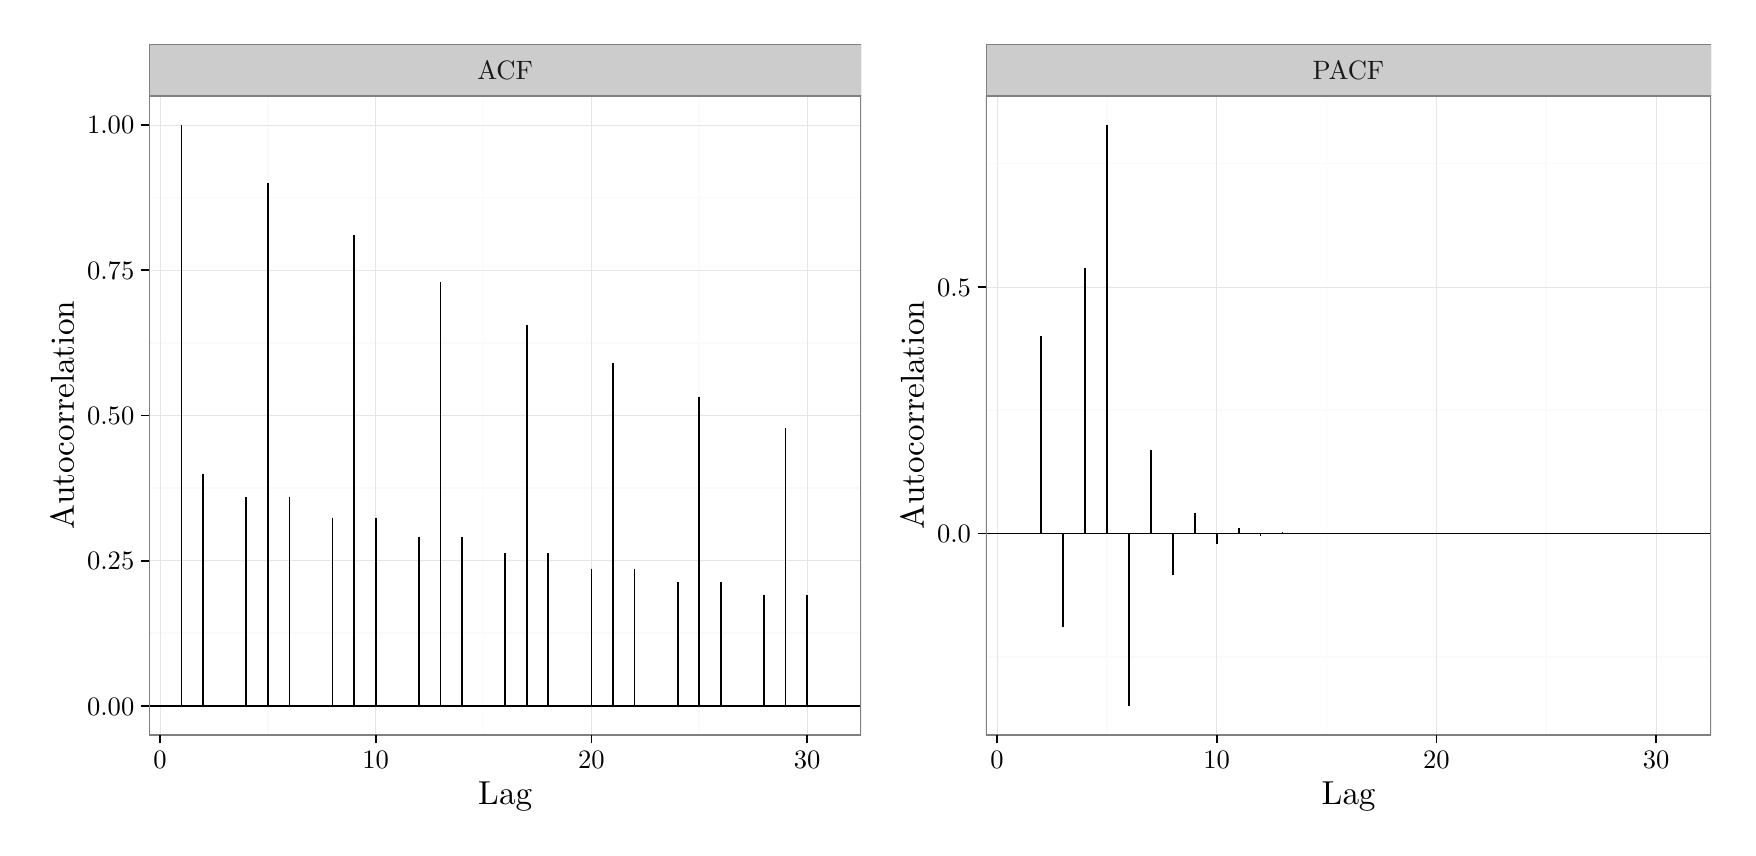
\begin{tikzpicture}[x=1pt,y=1pt]
\definecolor{fillColor}{RGB}{255,255,255}
\path[use as bounding box,fill=fillColor,fill opacity=0.00] (0,0) rectangle (614.29,289.08);
\begin{scope}
\path[clip] (  0.00,  0.00) rectangle (307.15,289.08);
\definecolor{drawColor}{RGB}{255,255,255}
\definecolor{fillColor}{RGB}{255,255,255}

\path[draw=drawColor,line width= 0.6pt,line join=round,line cap=round,fill=fillColor] ( -0.00,  0.00) rectangle (307.15,289.08);
\end{scope}
\begin{scope}
\path[clip] ( 43.93, 33.48) rectangle (301.15,264.47);
\definecolor{fillColor}{RGB}{255,255,255}

\path[fill=fillColor] ( 43.93, 33.48) rectangle (301.15,264.47);
\definecolor{drawColor}{gray}{0.98}

\path[draw=drawColor,line width= 0.6pt,line join=round] ( 43.93, 70.23) --
	(301.15, 70.23);

\path[draw=drawColor,line width= 0.6pt,line join=round] ( 43.93,122.72) --
	(301.15,122.72);

\path[draw=drawColor,line width= 0.6pt,line join=round] ( 43.93,175.22) --
	(301.15,175.22);

\path[draw=drawColor,line width= 0.6pt,line join=round] ( 43.93,227.72) --
	(301.15,227.72);

\path[draw=drawColor,line width= 0.6pt,line join=round] ( 86.80, 33.48) --
	( 86.80,264.47);

\path[draw=drawColor,line width= 0.6pt,line join=round] (164.74, 33.48) --
	(164.74,264.47);

\path[draw=drawColor,line width= 0.6pt,line join=round] (242.69, 33.48) --
	(242.69,264.47);
\definecolor{drawColor}{gray}{0.90}

\path[draw=drawColor,line width= 0.2pt,line join=round] ( 43.93, 43.98) --
	(301.15, 43.98);

\path[draw=drawColor,line width= 0.2pt,line join=round] ( 43.93, 96.47) --
	(301.15, 96.47);

\path[draw=drawColor,line width= 0.2pt,line join=round] ( 43.93,148.97) --
	(301.15,148.97);

\path[draw=drawColor,line width= 0.2pt,line join=round] ( 43.93,201.47) --
	(301.15,201.47);

\path[draw=drawColor,line width= 0.2pt,line join=round] ( 43.93,253.97) --
	(301.15,253.97);

\path[draw=drawColor,line width= 0.2pt,line join=round] ( 47.82, 33.48) --
	( 47.82,264.47);

\path[draw=drawColor,line width= 0.2pt,line join=round] (125.77, 33.48) --
	(125.77,264.47);

\path[draw=drawColor,line width= 0.2pt,line join=round] (203.72, 33.48) --
	(203.72,264.47);

\path[draw=drawColor,line width= 0.2pt,line join=round] (281.66, 33.48) --
	(281.66,264.47);
\definecolor{drawColor}{RGB}{0,0,0}

\path[draw=drawColor,line width= 0.6pt,line join=round] ( 43.93, 43.98) -- (301.15, 43.98);

\path[draw=drawColor,line width= 0.6pt,line join=round] ( 55.62,253.97) -- ( 55.62, 43.98);

\path[draw=drawColor,line width= 0.6pt,line join=round] ( 63.41,127.97) -- ( 63.41, 43.98);

\path[draw=drawColor,line width= 0.6pt,line join=round] ( 71.21, 43.98) -- ( 71.21, 43.98);

\path[draw=drawColor,line width= 0.6pt,line join=round] ( 79.00,119.57) -- ( 79.00, 43.98);

\path[draw=drawColor,line width= 0.6pt,line join=round] ( 86.80,232.97) -- ( 86.80, 43.98);

\path[draw=drawColor,line width= 0.6pt,line join=round] ( 94.59,119.57) -- ( 94.59, 43.98);

\path[draw=drawColor,line width= 0.6pt,line join=round] (102.39, 43.98) -- (102.39, 43.98);

\path[draw=drawColor,line width= 0.6pt,line join=round] (110.18,112.01) -- (110.18, 43.98);

\path[draw=drawColor,line width= 0.6pt,line join=round] (117.98,214.07) -- (117.98, 43.98);

\path[draw=drawColor,line width= 0.6pt,line join=round] (125.77,112.01) -- (125.77, 43.98);

\path[draw=drawColor,line width= 0.6pt,line join=round] (133.56, 43.98) -- (133.56, 43.98);

\path[draw=drawColor,line width= 0.6pt,line join=round] (141.36,105.21) -- (141.36, 43.98);

\path[draw=drawColor,line width= 0.6pt,line join=round] (149.15,197.06) -- (149.15, 43.98);

\path[draw=drawColor,line width= 0.6pt,line join=round] (156.95,105.21) -- (156.95, 43.98);

\path[draw=drawColor,line width= 0.6pt,line join=round] (164.74, 43.98) -- (164.74, 43.98);

\path[draw=drawColor,line width= 0.6pt,line join=round] (172.54, 99.09) -- (172.54, 43.98);

\path[draw=drawColor,line width= 0.6pt,line join=round] (180.33,181.75) -- (180.33, 43.98);

\path[draw=drawColor,line width= 0.6pt,line join=round] (188.13, 99.09) -- (188.13, 43.98);

\path[draw=drawColor,line width= 0.6pt,line join=round] (195.92, 43.98) -- (195.92, 43.98);

\path[draw=drawColor,line width= 0.6pt,line join=round] (203.72, 93.58) -- (203.72, 43.98);

\path[draw=drawColor,line width= 0.6pt,line join=round] (211.51,167.97) -- (211.51, 43.98);

\path[draw=drawColor,line width= 0.6pt,line join=round] (219.30, 93.58) -- (219.30, 43.98);

\path[draw=drawColor,line width= 0.6pt,line join=round] (227.10, 43.98) -- (227.10, 43.98);

\path[draw=drawColor,line width= 0.6pt,line join=round] (234.89, 88.62) -- (234.89, 43.98);

\path[draw=drawColor,line width= 0.6pt,line join=round] (242.69,155.57) -- (242.69, 43.98);

\path[draw=drawColor,line width= 0.6pt,line join=round] (250.48, 88.62) -- (250.48, 43.98);

\path[draw=drawColor,line width= 0.6pt,line join=round] (258.28, 43.98) -- (258.28, 43.98);

\path[draw=drawColor,line width= 0.6pt,line join=round] (266.07, 84.15) -- (266.07, 43.98);

\path[draw=drawColor,line width= 0.6pt,line join=round] (273.87,144.41) -- (273.87, 43.98);

\path[draw=drawColor,line width= 0.6pt,line join=round] (281.66, 84.15) -- (281.66, 43.98);

\path[draw=drawColor,line width= 0.6pt,line join=round] (289.46, 43.98) -- (289.46, 43.98);
\definecolor{drawColor}{gray}{0.50}

\path[draw=drawColor,line width= 0.6pt,line join=round,line cap=round] ( 43.93, 33.48) rectangle (301.15,264.47);
\end{scope}
\begin{scope}
\path[clip] ( 43.93,264.47) rectangle (301.15,283.08);
\definecolor{drawColor}{gray}{0.50}
\definecolor{fillColor}{gray}{0.80}

\path[draw=drawColor,line width= 0.2pt,line join=round,line cap=round,fill=fillColor] ( 43.93,264.47) rectangle (301.15,283.08);
\definecolor{drawColor}{gray}{0.10}

\node[text=drawColor,anchor=base,inner sep=0pt, outer sep=0pt, scale=  0.96] at (172.54,270.47) {ACF};
\end{scope}
\begin{scope}
\path[clip] (  0.00,  0.00) rectangle (614.29,289.08);
\definecolor{drawColor}{RGB}{0,0,0}

\node[text=drawColor,anchor=base east,inner sep=0pt, outer sep=0pt, scale=  0.96] at ( 38.53, 40.67) {0.00};

\node[text=drawColor,anchor=base east,inner sep=0pt, outer sep=0pt, scale=  0.96] at ( 38.53, 93.17) {0.25};

\node[text=drawColor,anchor=base east,inner sep=0pt, outer sep=0pt, scale=  0.96] at ( 38.53,145.67) {0.50};

\node[text=drawColor,anchor=base east,inner sep=0pt, outer sep=0pt, scale=  0.96] at ( 38.53,198.16) {0.75};

\node[text=drawColor,anchor=base east,inner sep=0pt, outer sep=0pt, scale=  0.96] at ( 38.53,250.66) {1.00};
\end{scope}
\begin{scope}
\path[clip] (  0.00,  0.00) rectangle (614.29,289.08);
\definecolor{drawColor}{RGB}{0,0,0}

\path[draw=drawColor,line width= 0.6pt,line join=round] ( 40.93, 43.98) --
	( 43.93, 43.98);

\path[draw=drawColor,line width= 0.6pt,line join=round] ( 40.93, 96.47) --
	( 43.93, 96.47);

\path[draw=drawColor,line width= 0.6pt,line join=round] ( 40.93,148.97) --
	( 43.93,148.97);

\path[draw=drawColor,line width= 0.6pt,line join=round] ( 40.93,201.47) --
	( 43.93,201.47);

\path[draw=drawColor,line width= 0.6pt,line join=round] ( 40.93,253.97) --
	( 43.93,253.97);
\end{scope}
\begin{scope}
\path[clip] (  0.00,  0.00) rectangle (614.29,289.08);
\definecolor{drawColor}{RGB}{0,0,0}

\path[draw=drawColor,line width= 0.6pt,line join=round] ( 47.82, 30.48) --
	( 47.82, 33.48);

\path[draw=drawColor,line width= 0.6pt,line join=round] (125.77, 30.48) --
	(125.77, 33.48);

\path[draw=drawColor,line width= 0.6pt,line join=round] (203.72, 30.48) --
	(203.72, 33.48);

\path[draw=drawColor,line width= 0.6pt,line join=round] (281.66, 30.48) --
	(281.66, 33.48);
\end{scope}
\begin{scope}
\path[clip] (  0.00,  0.00) rectangle (614.29,289.08);
\definecolor{drawColor}{RGB}{0,0,0}

\node[text=drawColor,anchor=base,inner sep=0pt, outer sep=0pt, scale=  0.96] at ( 47.82, 21.46) {0};

\node[text=drawColor,anchor=base,inner sep=0pt, outer sep=0pt, scale=  0.96] at (125.77, 21.46) {10};

\node[text=drawColor,anchor=base,inner sep=0pt, outer sep=0pt, scale=  0.96] at (203.72, 21.46) {20};

\node[text=drawColor,anchor=base,inner sep=0pt, outer sep=0pt, scale=  0.96] at (281.66, 21.46) {30};
\end{scope}
\begin{scope}
\path[clip] (  0.00,  0.00) rectangle (614.29,289.08);
\definecolor{drawColor}{RGB}{0,0,0}

\node[text=drawColor,anchor=base,inner sep=0pt, outer sep=0pt, scale=  1.20] at (172.54,  8.40) {Lag};
\end{scope}
\begin{scope}
\path[clip] (  0.00,  0.00) rectangle (614.29,289.08);
\definecolor{drawColor}{RGB}{0,0,0}

\node[text=drawColor,rotate= 90.00,anchor=base,inner sep=0pt, outer sep=0pt, scale=  1.20] at ( 16.66,148.97) {Autocorrelation};
\end{scope}
\begin{scope}
\path[clip] (307.15,  0.00) rectangle (614.29,289.08);
\definecolor{drawColor}{RGB}{255,255,255}
\definecolor{fillColor}{RGB}{255,255,255}

\path[draw=drawColor,line width= 0.6pt,line join=round,line cap=round,fill=fillColor] (307.15,  0.00) rectangle (614.29,289.08);
\end{scope}
\begin{scope}
\path[clip] (346.28, 33.48) rectangle (608.30,264.47);
\definecolor{fillColor}{RGB}{255,255,255}

\path[fill=fillColor] (346.28, 33.48) rectangle (608.29,264.47);
\definecolor{drawColor}{gray}{0.98}

\path[draw=drawColor,line width= 0.6pt,line join=round] (346.28, 61.79) --
	(608.30, 61.79);

\path[draw=drawColor,line width= 0.6pt,line join=round] (346.28,150.87) --
	(608.30,150.87);

\path[draw=drawColor,line width= 0.6pt,line join=round] (346.28,239.94) --
	(608.30,239.94);

\path[draw=drawColor,line width= 0.6pt,line join=round] (389.95, 33.48) --
	(389.95,264.47);

\path[draw=drawColor,line width= 0.6pt,line join=round] (469.35, 33.48) --
	(469.35,264.47);

\path[draw=drawColor,line width= 0.6pt,line join=round] (548.75, 33.48) --
	(548.75,264.47);
\definecolor{drawColor}{gray}{0.90}

\path[draw=drawColor,line width= 0.2pt,line join=round] (346.28,106.33) --
	(608.30,106.33);

\path[draw=drawColor,line width= 0.2pt,line join=round] (346.28,195.41) --
	(608.30,195.41);

\path[draw=drawColor,line width= 0.2pt,line join=round] (350.25, 33.48) --
	(350.25,264.47);

\path[draw=drawColor,line width= 0.2pt,line join=round] (429.65, 33.48) --
	(429.65,264.47);

\path[draw=drawColor,line width= 0.2pt,line join=round] (509.05, 33.48) --
	(509.05,264.47);

\path[draw=drawColor,line width= 0.2pt,line join=round] (588.45, 33.48) --
	(588.45,264.47);
\definecolor{drawColor}{RGB}{0,0,0}

\path[draw=drawColor,line width= 0.6pt,line join=round] (346.28,106.33) -- (608.30,106.33);

\path[draw=drawColor,line width= 0.6pt,line join=round] (366.13,177.59) -- (366.13,106.33);

\path[draw=drawColor,line width= 0.6pt,line join=round] (374.07, 72.40) -- (374.07,106.33);

\path[draw=drawColor,line width= 0.6pt,line join=round] (382.01,202.32) -- (382.01,106.33);

\path[draw=drawColor,line width= 0.6pt,line join=round] (389.95,253.97) -- (389.95,106.33);

\path[draw=drawColor,line width= 0.6pt,line join=round] (397.89, 43.98) -- (397.89,106.33);

\path[draw=drawColor,line width= 0.6pt,line join=round] (405.83,136.34) -- (405.83,106.33);

\path[draw=drawColor,line width= 0.6pt,line join=round] (413.77, 91.46) -- (413.77,106.33);

\path[draw=drawColor,line width= 0.6pt,line join=round] (421.71,113.75) -- (421.71,106.33);

\path[draw=drawColor,line width= 0.6pt,line join=round] (429.65,102.62) -- (429.65,106.33);

\path[draw=drawColor,line width= 0.6pt,line join=round] (437.59,108.18) -- (437.59,106.33);

\path[draw=drawColor,line width= 0.6pt,line join=round] (445.53,105.40) -- (445.53,106.33);

\path[draw=drawColor,line width= 0.6pt,line join=round] (453.47,106.79) -- (453.47,106.33);

\path[draw=drawColor,line width= 0.6pt,line join=round] (461.41,106.10) -- (461.41,106.33);

\path[draw=drawColor,line width= 0.6pt,line join=round] (469.35,106.45) -- (469.35,106.33);

\path[draw=drawColor,line width= 0.6pt,line join=round] (477.29,106.27) -- (477.29,106.33);

\path[draw=drawColor,line width= 0.6pt,line join=round] (485.23,106.36) -- (485.23,106.33);

\path[draw=drawColor,line width= 0.6pt,line join=round] (493.17,106.32) -- (493.17,106.33);

\path[draw=drawColor,line width= 0.6pt,line join=round] (501.11,106.34) -- (501.11,106.33);

\path[draw=drawColor,line width= 0.6pt,line join=round] (509.05,106.33) -- (509.05,106.33);

\path[draw=drawColor,line width= 0.6pt,line join=round] (516.99,106.33) -- (516.99,106.33);

\path[draw=drawColor,line width= 0.6pt,line join=round] (524.93,106.33) -- (524.93,106.33);

\path[draw=drawColor,line width= 0.6pt,line join=round] (532.87,106.33) -- (532.87,106.33);

\path[draw=drawColor,line width= 0.6pt,line join=round] (540.81,106.33) -- (540.81,106.33);

\path[draw=drawColor,line width= 0.6pt,line join=round] (548.75,106.33) -- (548.75,106.33);

\path[draw=drawColor,line width= 0.6pt,line join=round] (556.69,106.33) -- (556.69,106.33);

\path[draw=drawColor,line width= 0.6pt,line join=round] (564.63,106.33) -- (564.63,106.33);

\path[draw=drawColor,line width= 0.6pt,line join=round] (572.57,106.33) -- (572.57,106.33);

\path[draw=drawColor,line width= 0.6pt,line join=round] (580.51,106.33) -- (580.51,106.33);

\path[draw=drawColor,line width= 0.6pt,line join=round] (588.45,106.33) -- (588.45,106.33);

\path[draw=drawColor,line width= 0.6pt,line join=round] (596.39,106.33) -- (596.39,106.33);
\definecolor{drawColor}{gray}{0.50}

\path[draw=drawColor,line width= 0.6pt,line join=round,line cap=round] (346.28, 33.48) rectangle (608.29,264.47);
\end{scope}
\begin{scope}
\path[clip] (346.28,264.47) rectangle (608.30,283.08);
\definecolor{drawColor}{gray}{0.50}
\definecolor{fillColor}{gray}{0.80}

\path[draw=drawColor,line width= 0.2pt,line join=round,line cap=round,fill=fillColor] (346.28,264.47) rectangle (608.29,283.08);
\definecolor{drawColor}{gray}{0.10}

\node[text=drawColor,anchor=base,inner sep=0pt, outer sep=0pt, scale=  0.96] at (477.29,270.47) {PACF};
\end{scope}
\begin{scope}
\path[clip] (  0.00,  0.00) rectangle (614.29,289.08);
\definecolor{drawColor}{RGB}{0,0,0}

\node[text=drawColor,anchor=base east,inner sep=0pt, outer sep=0pt, scale=  0.96] at (340.88,103.02) {0.0};

\node[text=drawColor,anchor=base east,inner sep=0pt, outer sep=0pt, scale=  0.96] at (340.88,192.10) {0.5};
\end{scope}
\begin{scope}
\path[clip] (  0.00,  0.00) rectangle (614.29,289.08);
\definecolor{drawColor}{RGB}{0,0,0}

\path[draw=drawColor,line width= 0.6pt,line join=round] (343.28,106.33) --
	(346.28,106.33);

\path[draw=drawColor,line width= 0.6pt,line join=round] (343.28,195.41) --
	(346.28,195.41);
\end{scope}
\begin{scope}
\path[clip] (  0.00,  0.00) rectangle (614.29,289.08);
\definecolor{drawColor}{RGB}{0,0,0}

\path[draw=drawColor,line width= 0.6pt,line join=round] (350.25, 30.48) --
	(350.25, 33.48);

\path[draw=drawColor,line width= 0.6pt,line join=round] (429.65, 30.48) --
	(429.65, 33.48);

\path[draw=drawColor,line width= 0.6pt,line join=round] (509.05, 30.48) --
	(509.05, 33.48);

\path[draw=drawColor,line width= 0.6pt,line join=round] (588.45, 30.48) --
	(588.45, 33.48);
\end{scope}
\begin{scope}
\path[clip] (  0.00,  0.00) rectangle (614.29,289.08);
\definecolor{drawColor}{RGB}{0,0,0}

\node[text=drawColor,anchor=base,inner sep=0pt, outer sep=0pt, scale=  0.96] at (350.25, 21.46) {0};

\node[text=drawColor,anchor=base,inner sep=0pt, outer sep=0pt, scale=  0.96] at (429.65, 21.46) {10};

\node[text=drawColor,anchor=base,inner sep=0pt, outer sep=0pt, scale=  0.96] at (509.05, 21.46) {20};

\node[text=drawColor,anchor=base,inner sep=0pt, outer sep=0pt, scale=  0.96] at (588.45, 21.46) {30};
\end{scope}
\begin{scope}
\path[clip] (  0.00,  0.00) rectangle (614.29,289.08);
\definecolor{drawColor}{RGB}{0,0,0}

\node[text=drawColor,anchor=base,inner sep=0pt, outer sep=0pt, scale=  1.20] at (477.29,  8.40) {Lag};
\end{scope}
\begin{scope}
\path[clip] (  0.00,  0.00) rectangle (614.29,289.08);
\definecolor{drawColor}{RGB}{0,0,0}

\node[text=drawColor,rotate= 90.00,anchor=base,inner sep=0pt, outer sep=0pt, scale=  1.20] at (323.81,148.97) {Autocorrelation};
\end{scope}
\end{tikzpicture}
